\documentclass[12pt,a4paper, oneside]{article}
\usepackage[utf8]{inputenc}
\usepackage[T1]{fontenc}
\usepackage[english,german]{babel}
\usepackage[style=german]{csquotes}
\usepackage{graphicx}

\author{Uni Oldenburg, SWP2020 Gruppe A}

\begin{document}

    \begin{titlepage}
        \pagestyle{empty}
        \begin{center}

            \begin{figure}[h]
                \centering
                
\includegraphics[width=0.35\textwidth]{../img/Logo.jpg}
            \end{figure}

            \bigskip \bigskip \noindent
            \textsc{\textbf{\LARGE Softwareprojekt:}} \par \bigskip \noindent
            \textsc{\textbf{\LARGE Projekttagebuch}}


            \par \bigskip \bigskip \bigskip \bigskip \bigskip \noindent
            {\Large Gruppe A} \par \medskip \noindent

            \par \bigskip \bigskip \bigskip \bigskip \bigskip \bigskip \noindent
            \textit{\Large Wintersemester 2020/21 und} \par \noindent
            \textit{\Large Sommersemester 2021}

            \par \bigskip \bigskip \bigskip \bigskip \bigskip \bigskip \noindent
            \par \bigskip \bigskip \bigskip \noindent
            {\Large Sprintanalyse} \par \medskip \noindent

        \end{center}
    \end{titlepage}

    \tableofcontents
    \pagebreak


    \section{Sprinttagebuch: Sprint-Nr. 7}
    \underline{Name des Sprints:}
    \\
    Sprint 7: Ort der Finsternis

    \noindent
    \\
    \underline{Zeitraum des Sprints:}
    \\
    11. März 2021 - 30. März 2021

    \noindent
    \\
    \underline{Ziel des Sprints:}
    \\
    Grundlagen für Spielfeldinteraktion, UX, Refactoring


    \noindent
    \\
    \underline {Team:}
    \\
    Sven Ahrens, Alwin Bossert, Aldin Dervisi, Marvin Drees, Mario Fokken,
    Timo Gerken, Finn Haase, Temmo Junkhoff, Maximilian Lindner, Steven Luong, Phillip-André Suhr, Eric Vuong


    \section{Vorgänge}

    \begin{itemize}

        \item SWP2020A-126: ANmi, dass zu Beginn einer Partie immer ein zufällig generiertes Spielfeld vorliegt, damit jede Partie unterschiedlich ist. (2 Story Points)

        \item SWP2020A-135: ANmi, dass das System nach dem Würfeln automatisch die korrekten Ressourcen an alle Spieler verteilt (4 Story Points)

        \item SWP2020A-144: ANmi überall entfernt werden, falls meine Verbindung abbricht (4 Story Points)

        \item SWP2020A-158: AEmi, dass das Spielfeld bei Anklicken bestimmt, auf was (welche(s) Hex/Siedlung/Straße) geklickt wurde (11 Story Points)

        \item SWP2020A-175: Bericht für Sprint 6 erstellen (2 Story Points)

        \item SWP2020A-176: ANmi, dass ein Spieler beim Erreichen von 10 Siegpunkten als Gewinner bekanntgegeben und die Partie beendet wird. (2 Story Points)

        \item SWP2020A-193: Die IllegalArgumentException von createGame im GameManagement wird nicht abgefangen (1 Story Point)

        \item SWP2020A-195: ANmi sehen wieviele Karten die anderen Spieler auf der Hand haben (2 Story Points)

        \item SWP2020A-200: ANmi, dass das Spielfeld sich der Größe des Lobbyfensters anpasst, wenn diese verändert wird (2 Story Points)

        \item SWP2020A-201: AEmi meiner Partie Dummy-User hinzufügen können, die nur würfeln und "End Turn" drücken (2 Story Points)

        \item SWP2020A-202: I18n für Dialogfenster (1 Story Point)

        \item SWP2020A-203: ANmi die Möglichkeit haben, ein Gegenangebot stellen zu können, falls mir das gestellte Angebot nicht gefällt (1 Story Point)

        \item SWP2020A-206: ANmi im Chat sehen können, welche Ressourcen zwei Spieler miteinander getauscht haben (2 Story Points)

        \item SWP2020A-209: ANmi vor Start einer Session im Lobbyfenster einige Einstellungen nutzen können (3 Story Points)

        \item SWP2020A-210: In (fast) allen Tests die Asserts umdrehen (2 Story Points)

        \item SWP2020A-212: Statt Iteration über getInventories() sollte getInventory(getPlayer(User)) genutzt werden (1 Story Point)

        \item SWP2020A-217: LobbyPresenter refactoren/abstrahieren falls möglich (2 Story Points)

        \item SWP2020A-218: ANmi meine Nutzerdaten (Name, Passwort, EMail) in einem Fenster ändern können (2 Story Points)

        \item SWP2020A-222: Alle Fenster sollen bei Vergrößerung ihre Elemente entsprechend anpassen, dass das Layout noch vernünftig aussieht (2 Story Points)

        \item SWP2020A-224: Chatnachrichten mit Enter senden können (1 Story Point)

        \item SWP2020A-248: UserOrDummy-Parsing in CommandService integrieren (0 Story Points)

    \end{itemize}

    \newpage

    \subsection{Sprinterfolg}
    \begin{figure}[h]
        \centering
        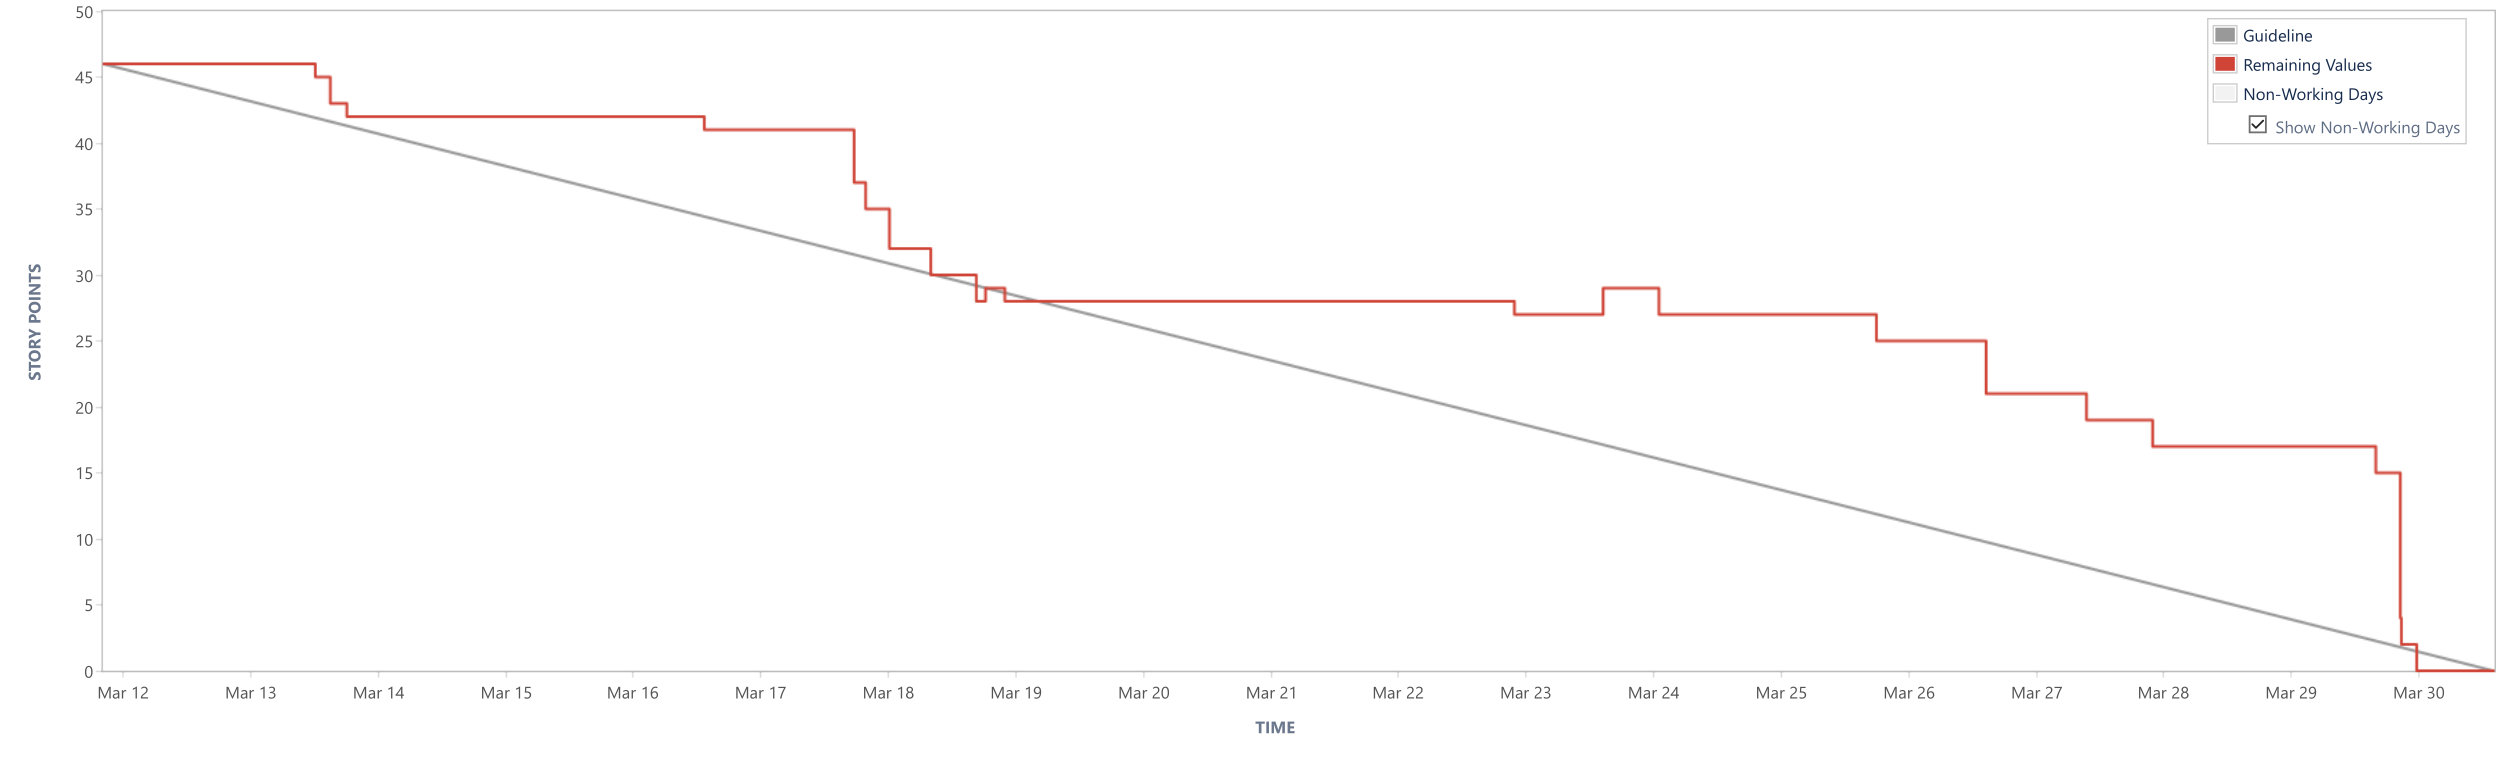
\includegraphics[width=\textwidth, height=5cm]{../img/sprint_07/Burndown-Sprint7.png}
        \caption{Burndown-Diagramm Sprint 7}
        \label{fig: Burndown-Sprint7}
    \end{figure}
    \noindent
    Dieser Sprint ist im Vergleich zum Vorgänger zwar mit weniger Storypoints versehen, aber das rührt daher,
    dass wir uns beim Bewerten der Tasks zurückgehalten haben und eher weniger Punkte verteilt haben, obwohl
    der Umfang ähnlich war.
    Die wohl am hervorstechendeste Task ist die \textit{SWP2020A-158: AEmi, dass das Spielfeld bei Anklicken bestimmt, auf was (welche(s) Hex/Siedlung/Straße) geklickt wurde} mit ganzen 11 Punkten, welche auch den spürbarsten Fortschritt
    im Client brachte.

    \subsection{Sprintprobleme bzw. Hindernisse}
    Als Hindernis ist in der Zeit zwischen dem 19.03. und 25.03
    die Klausur im Modul Softwaretechnik anzumerken, dadurch konnten
    wir uns nicht so eng an der Guideline halten.

    \newpage


    \section{Erkenntnis aus der Retrospektive}
    Folgende Erkenntnisse ergaben sich aus der Retrospektive:\\

    \underline{Start:}\\

    \underline{Stop:}
    \begin{itemize}
        \item Reviews zeitnah (erste Review binnen 48 Stunden) erledigen
    \end{itemize}\\

    \underline{Weiter so:}
    \begin{itemize}
        \item Ansprechbar sein auf Discord (max. 2 Tage für Antworten)
        \item Bei Nachbesserungswünschen immer "Benötigt Nachbesserung" anklicken
        \item Reviews weiterhin gründlich durchführen
        \item Pair-Programming
    \end{itemize}

    \newpage


    \section{Sonstige Anmerkungen}

    Bei diesem Sprint ist die zeitliche Beschränkung der Teammitglieder, aufgrund der parallelen Klausurenphase der Nachschreibklausuren, anzumerken.
    Außerdem wurden die Tasks \textit{SWP2020A-224: Chatnachrichten mit Enter senden können}, welche mit einem Story Point geschätzt wurde, sowie die \textit{SWP2020A-248: UserOrDummy-Parsing in CommandService integrieren} , welche mit 0 Story Points geschätzt wurde, später im laufenden Sprint nachgezogen.
    Des Weiteren wurden die Reviews ausführlicher gemacht, wodurch einige PRs öfter aktualisiert wurden und somit länger
    bis zum Merge brauchten.


    \section{Fazit}
    Insgesamt lässt sich sagen, dass das Sprintziel von diesem Sprint erreicht wurde und alle Aufgaben rechtzeitig erfolgreich, laut der Definition of Done, abgeschlossen wurden.
    Nach einer zeitlich bedingten Phase in der die Tasks brach, lagen konnte das Team sich wieder aufraffen und somit das angestrebte Sprintziel erreichen.
    Die zeitlich parallele zweite Klausurenphase wird zu der Regenerationsphase des Teams auch ihren Beitrag geleistet haben.
    Mit insgesamt 46 Story Points (mit einberechnen der nachgezogenen Tasks) gehört dieser Sprint nicht zu den umfangreichsten bisher, was sich wohl auch durch unser angepasstes Schätzverhalten erklären lässt.
    Trotzdem waren alle Teammitglieder die meiste Zeit durchgehend mit Arbeit versorgt.

\end{document}
